% !TEX root = ../thesis.tex
\chapter{Evaluation} \label{evaluation}
\section{Experiment} \label{experiment}
Let us prepare experiment to test our models.
We have prepared three models to create a prediction.
Data from section~\ref{sec:preprocessing} was used to predict the income for the year 2020.
We used Matlab to calculate linear regression analysis, polynomial regression analysis and prepare prediction application with Customer behavior HMM.
From each process we got real income for the year 2020, which were subsequently compared in Evaluation section~\ref{evaluation}.
Firstly we solved linear regression for model.
The second one was polynomial model.
At the last one we solved Customer behavior HHM as submodel combination in $P = (Y_n \in A|X_n = x_n)$.
At a first glance we can see that the results from the models are different.
The first linear model with trigonometric function is not satisfying in real income results, but on the other hand was produced a very interesting result for trend prediction.
In~contrast with polynomial model which has much better results in absolut income results, but much worse in trend prediction.\\
We compared prediction period and for each we calculate aberration against real store income from 2020.
Let us see our experiment in detail description and then see results in Evaluation section~\ref{evaluation} and Summary section~\ref{summary}.\\
\subsection{Preprocessing of input data} \label{sec:preprocessing}
The data comes from Megaplay s.r.o online stores and should have to be\\ anonymized \footnote{Data anonymization is a type of information sanitization whose intent is privacy protection.
It is the process of either encrypting or removing personally identifiable information from data sets, so that
the people whom the data describe remain anonymous.} and pseudonymized \footnote{Pseudonymization is a data management
and de-identification procedure by which personally identifiable information fields within a data record are replaced
by one or more artificial identifiers, or pseudonyms.} to keep legal notice of~\cite{gdpr}.
Then we should utilize data to utilized inputs.
This prepared data will serve for baseline (Linear and polynomial models) and our prediction Customer behavior HMM.\\
\\
\textbf{Average day visitors for a predicted month}\\
This value was calculated from anonymized users data from Google Analytics tool using their prediction mechanism to get number of future users based on the number of previous visitors.\\
\\
\textbf{Perceived value for psychology model} \label{perceived}\\
This variable is needed for loyalty model (see section~\ref{subsec:model_loyalty}) and comes from an open e-commerce comparison data provided by Heureka.cz/Heureka.sk internal tool.\\
\\
\textbf{Number of orders 2018 - 2019}\\
Number of orders we get from shopycrm.com tool used in Megaplay s.r.o to manage their business processes and also store all needed data.\\
\\
\textbf{Unique products sell}\\
This variable is used in Psychology model (see section~\ref{subsec:model_psychology}) for Price aspect calculation~\ref{eq:17}.\\
\\
\textbf{Customer satisfaction} \label{customerSat}\\
This value is provided by Heureka open data, and it's a calculated value from the customer reviews of the store.\\
\\
\textbf{Margin}\\
The retail margin percentage measures the retail margin as a percentage of the retail price.
This measurement gives you a context for the retail margin.
For example, if you have a 5~€ retail margin on two different products, but one costs 150~€ and next one costs 10~€, the second product would have a much higher retail margin percentage.\\
\\
\textbf{Number of product order each day $Q_i$}\\
This is a calculated value from shopycrm.com about the number of product orders for each one.
It's used in Psychology model~\ref{subsec:model_psychology}. \\
\\
\textbf{Quality index $Q_1$}\\
This is vendor quality index provided by Heureka open data.
This is a power/strength of the store.
Higher number means that for a customer it is more difficult to leave the store and go to another online store.\\
\\
\textbf{Vendor coefficients $\beta, \gamma, \delta$} \label{vendorCoeff}\\
This three coefficients are used as weights for vendor model~\ref{subsec:model_vendors} and were set with cooperation with Megaplay s.r.o owner for their industry.
It represents the relation between vendor prices and vendor quality.\\
\\
\subsection{Models for prediction} \label{subsec:calculate_models}
As a baseline for our model linear and polynomial fitting (see section~\ref{sec:regression}) will be used.
There are first two models which have to be solved.
The last one is our new Customer behavior HMM:\\
\begin{itemize}
    \item $f(x) = a(\sin(x-\pi))+b((x-10)^2)+c,$
    \item $f(x) = p_1x^4 + p_2x^3 + p_3x^2 + p_4x + p_5,$\\
    \item $P = \left(
    \begin{pmatrix}
        V_{xy} & V_{xy} & V_{xy} \\
        \alpha + \beta & \alpha + \beta & \alpha + \beta \\
        \frac{R + Z}{Z} & \frac{R + Z}{Z} & \frac{R + Z}{Z}
    \end{pmatrix}|
    \begin{pmatrix}
        l & m & k \\
        l & m & k \\
        l & m & k
    \end{pmatrix}
    \right)$\\
    \\
\end{itemize}\\
\\
\textbf{Using random values for Customer behavior HMM}\\
In our model we use randomly generated variables which were used to simulate situations from real store where the user can compare one store to another one in the different situation.
In other stores the situation should be better or worse to actual store.
To improve the results, it should be better to use data from real competitors from each trade, but it is not easy to obtain them.
This random variables are used as a simplification of that situation.\\
\\
All input data and models were prepared, so the prediction can be simulated.
Let us use data prepared in section~\ref{sec:preprocessing} and calculate prediction income from identified models.
\subsection{Comparison criteria} \label{subsec:result_metodology}
Finally we define the method to compare our models results.
Absolute number of income value prediction should not be important for the store owners because of that we calculated the aberration for each month
prediction and then we easily calculate quarterly and yearly results.
The sum of squared errors (SSE), defined by:
$$SSE = \sum^n_{i=1}w_i(y_i - \overline{y_i})^2,$$
between the fitting models and the used data serves as the fitting criterion,
with values closer to $0$ indicating a smaller random error component of the model.
Also some other quality measures were evaluated, \textit{i.e.} the R-square from interval $[0,\ 1]$,
that indicates the proportion of variance satisfactory explained by the fitting-model (\textit{e.g.}  R-square $= 0.7325$ means
that the fit explains $73.25\%$ of the total variation in the data about the average);
R-square is defined as the ratio of the sum of squares of the regression (SSR) and the total sum of squares (SST).
SSR is defined as
$$SSR = \sum_{i=1}^nw_i(\overline{y_i} - \overline{y_i})^2.$$
SST is also called the sum of squares about the mean, and is defined as
$$SST = \sum_{i=1}^nw_i(y_i - \overline{y})^2,$$
where SST = SSR + SSE. Givenm these definition, R-square is expressed as
$$\frac{SSR}{SST} = 1 - \frac{SSE}{SST}.$$
The adjusted R-square statistic, with values smaller or equal to $1$, where values closer to $1$ indicate a better fit; the root mean squared error (RMSE):\\
$$RMSE = s = \sqrt{\frac{SSE}{v}}$$
with values closer to $0$ indicating a fit more useful for prediction~\cite{cftool}.
\subsection{Results} \label{experimentResults}
To get prediction results identified parameters and coefficients were calculated.
Then identified models were used to get prediction income in 2020 and 2021.
Models from section~\ref{subsec:calculate_models} were fitted on the real data from year 2018 and 2019.
On the figure~\ref{plot} is graphical presentation of data and our models is shown.
It turned out that the linear model (blue line), is not directly corresponding to the data, but it is copying the trend of the income (red line),
polynomial model (green line) returns better results that previous one.
The best results returned from Customer behavior HMM (violet line).
can be seen especially on figure~\ref{results} with predicted data to 2020.
\begin{figure}[h!]
    \begin{center}
        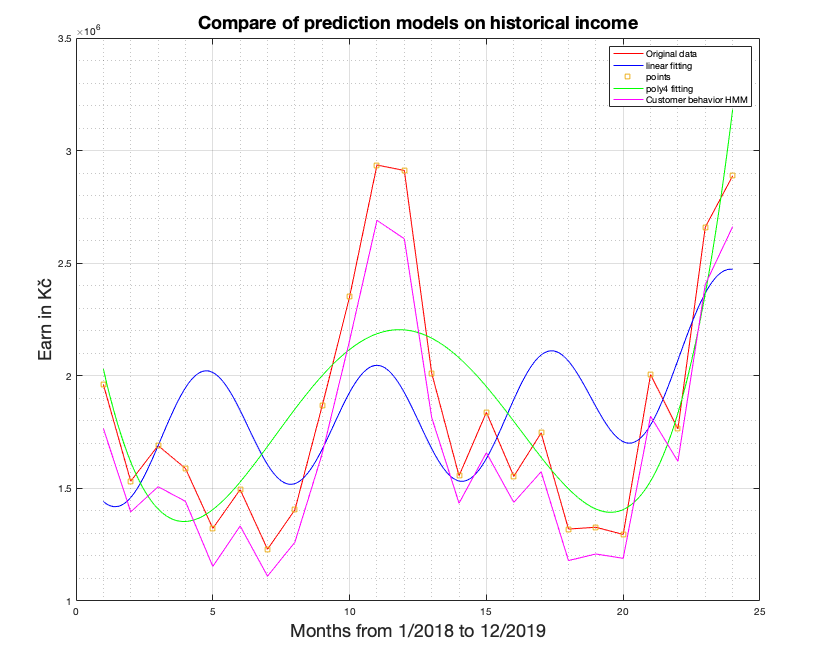
\includegraphics[width=140mm]{plot.png}
    \end{center}
    \caption{Fitting the model on real income from 2018 and 2019}
    \label{plot}
\end{figure}\\
With Megaplay s.r.o employees and heureka e-comerce tool the probability weights were set in form of vector for
Customer behavior HMM which tells about probabilities for each hidden states described in section~\ref{sec:submodels}
Vector have to be updated to square matrix which is used in Customer behavior HMM.
Other industry dependent weights and coefficients were set with Megaplay s.r.o employees, based on their data and experiences as in table~\ref{megaplay_data}.\\
Linear and polynomial models were identified with matlab Curve Fitting toolbox, see parameters in the table~\ref{parameters}.
\newpage
\begin{table}[h!]
    \begin{center}
        \begin{tabular}{ | l | c |}
            \hline
            {\textbf{Variable name}} & \textbf{Result}\\
            \hline
            average day visitors for a predicted month $U_a$& 2357 \\
            perceived value for psychology model & 0.87 \\
            number of orders 2018 - 2019 $O_c$ & 26 530 \\
            Unique products sell $U_p$ & 11048\\
            Customer satisfaction & 90\%\\
            Margin & 0.27\\
            $Q_i$ & 4.12\\
            $Q_1$ & 0.94\\
            Vendor coefficients: & \\
            $\beta$ & 0.7\\
            $\gamma$ & 0.7\\
            $\delta$ & 0.85\\
            \hline
            number of visitors 1/2020 & $31 * U_a$\\
            average earn per order & $\sum Income / O_c$\\
            \overline{Q} & $1/U_p * (U_p/ O_c)$\\
            \overline{P} & $1/U_p * margin$\\
            trust & $1/O_c * O_c/U_a$\\
            \hline
        \end{tabular}
    \end{center}
    \caption{Coefficient and calculated values data from Megaplay s.r.o for Customer behavior HMM}
    \label{megaplay_data}
\end{table}\\
\\
\begin{table}[h!]
    \begin{center}
        \begin{tabular}{ | l | l | l |}
            \hline
            \textbf{linear model} & \textbf{polynomial model} & \textbf{Customer behavior HMM}\\
            \hline
            \makecell{$a =2.978.10^5$\\$b = 1687$\\$c = 1.753.10^6$} & \makecell{$p_1 = 225.1$\\$p_2 = -1.059.10^4$\\$p_3 =1.596.10^5$\\$p_4 = -8.205.10^5$\\$p_5 = 2.702.10^6$} & \makecell{$l = 1/2$\\$m = 1/3$\\$k = 1/9$}\\
            \hline
        \end{tabular}
    \end{center}
    \caption{Identified parameters for models}
    \label{parameters}
\end{table}\\
On the figure~\ref{results} prediction results are shown.
For the year 2021 the models are compared with the real income and we can see that the polynomial and Customer behavior HMM model
get good results, in the opposite of results of linear model prediction.

\begin{figure}[h!]
    \begin{center}
        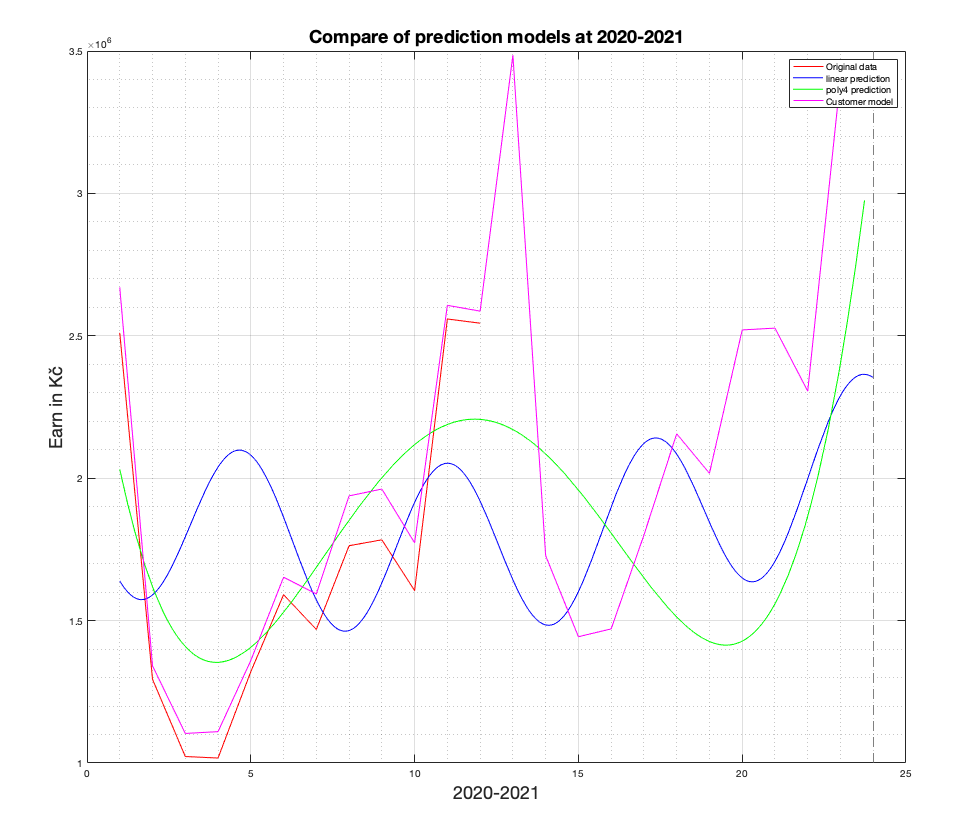
\includegraphics[width=140mm]{results.png}
    \end{center}
    \caption{Prediction from models for years 2020-2021, with real income for 2020.}
    \label{results}
\end{figure}\\
In the graphical view we saw that all our models copy the income, but some of them are easier to calculate, this differences you can see described in Summary (see section~\ref{summary}).
Lets use our defined methodology (see section~\ref{subsec:result_metodology}) to compare our models.
As it given in the table~\ref{compare} our Customer behavior HMM return best results from all tested models.
\begin{table}[h!]
    \begin{center}
        \begin{tabular}{ | l | c | c | c |}
            \hline
            & \textbf{linear model} & \textbf{polynomial model} & \textbf{Customer behavior HMM}\\
            \hline
            \textbf{SSE} & 5,165.10^{12} & 2,534.10^{12} & 1,583.10^{11} \\
            \textbf{R-square} & 0,2162 & 0,6154 & 0,95 \\
            \textbf{RMSE} & 4,959.10^5 & 3,652.10^5 & 1,149.10^5\\
            \hline
        \end{tabular}
    \end{center}
    \caption{Compare goodness-of-fit for models.}
    \label{compare}
\end{table}\\
In the table~\ref{Compare results} calculated percentage aberration from real income in the year 2021 are given.
We saw that there is no model which returned best results in every month, but in most months the best results are offered by Customer behavior HMM.
\begin{table}[h!]
    \begin{center}
        \begin{tabular}{ | l | c | c | c |}
            \hline
            {\textbf{Month}} & \textbf{Linear model} & \textbf{Polynomial model} & \textbf{Customer behavior HMM}\\
            \hline
            1/2021 & 53 & 24 &  7\\
            2/2021 & 23 & 31 & 6\\
            3/2021 & 71 & 38 & 7\\
            4/2021 & 101 & 38 & 13\\
            5/2021 & 57 & 6 & 4\\
            6/2021 & 17 & 5 & 3\\
            7/2021 & 5 & 13 & 7\\
            8/2021 & 20 & 5 & 11\\
            9/2021 & 11 & 11 & 9\\
            10/2021 & 20 & 31 & 10\\
            11/2021 & 25 & 17 & 2\\
            12/2021 & 32 & 16 & 3\\
            \hline
        \end{tabular}
    \end{center}
    \caption{Compare aberration (\%) from real income 2020}
    \label{Compare results}
\end{table}\\
Calculated result per each quarter in 2020 can bee seen in the table~\ref{qResults} showing to us the oscillation of prediction.
\begin{table}[h!]
    \begin{center}
        \begin{tabular}{ | l | c | c | c |}
            \hline
            & \textbf{Linear model} & \textbf{Polynomial model} & \textbf{Customer behavior HMM}\\
            \hline
            1Q (\%) & 49,24 & 30,81 & 6,42\\
            2Q (\%) & 58,24 & 15,00 & 6,50\\
            3Q (\%) & 12,15 & 9,64 & 9,25\\
            4Q (\%) & 25,59 & 21,21 & 4,89\\
            \hline
        \end{tabular}
    \end{center}
    \caption{Quarterly results}
    \label{qResults}
\end{table}\\
\section{Matlab Live script application} \label{livescript}
Implementation of our experiment created in Matlab with results explanations enriched with Live script application with dynamic weights setting is described in this section.
\subsection{Used software, libraries and predefined functions} \label{subsec:libraries}
\textbf{Matlab 2020a}\\
MATLAB (matrix laboratory) is a fourth-generation high-level programming language and interactive environment for numerical
computation, visualization and programming developed by MathWorks.\\
\\
\textbf{Matlab LiveScript}~\cite{livescript}\\
MATLAB live scripts and live functions are interactive documents that combine MATLAB code with formatted text, equations,
and images in a single environment called the Live Editor.
In addition, live scripts store and display output alongside the code that creates it.\\
Use live scripts and functions to:\\
\begin{itemize}
    \item Visually explore and analyze problems.
    \item Share richly formatted, executable narratives.
    \item Create interactive lectures for teaching.
\end{itemize}\\
\\
\textbf{Matlab Curve Fitting Tool}\\
The Curve Fitting Toolbox provides a collection of GUIs and M-files.
With the toolbox we are able to data preprocessing such as sectioning and smoothing, parametric and nonparametric data fitting,
and also fit statistics which assist us in determining the goodness of fit,analysis capabilities such as extrapolation, differentiation, and integration.
A graphical environment allows you to explore and analyze data sets and fits visually and numerically.\\
\textbf{hhmgenerate~\cite{hhmgenerate}}\\
The function $hmmgenerate$ begins with the model in state 1 at step 0, prior to the first emission.
The model then makes a transition to state $i_1$, with probability $T_{1i_1}$, and generates an emission $a_k_1$ with probability $E_{i_1k_11}$.
$hmmgenerate$ returns $i_1$ as the first entry of states, and $a_k_1$ as the first entry of seq.
$[seq,states] = hmmgenerate(len,TRANS,EMIS)$ takes a known Markov model, specified by transition probability matrix $TRANS$ and emission probability matrix $EMIS$,
and uses it to generate:\\
\begin{itemize}
    \item A random sequence seq of emission symbols.
    \item A random sequence states of states.
\end{itemize}
The length of both $seq$ and $states$ is $len$.
$TRANS(i,j)$ is the probability of transition from state $i$ to state $j$.
$EMIS(k,l)$ is the probability that symbol $l$ is emitted from state $k$.\\
\\
\textbf{hhmviterbi}~\cite{hhmviterbi}\\
The function $hmmviterbi$ begins with the model in state 1 at step 0, prior to the first emission.
hmmviterbi computes the most likely path based on the fact that the model begins in state 1.
$STATES = hmmviterbi(seq,TRANS,EMIS)$ given a $sequence, seq$, calculates the most likely path through the hidden Markov model
specified by transition probability matrix, $TRANS$, and emission probability matrix $EMIS$. $TRANS(i,j)$ is the probability of transition from state $i$ to state $j$.
$EMIS(i,k)$ is the probability that symbol $k$ is emitted from state $i$.\\
\\
\textbf{shopycrm.com}\\
Online CRM application focused on e-commerce stores which provides all store workflows and get precalculated data which
we will use for our models to simplify the prediction calculation.
\subsection{Fitting models and prediction} \label{fitting}
Let us use Matlab Curve fitting tool to solve our linear and polynomial models as you can see on figure~\ref{cftool},
this predefined tool calculates coefficients and then the prediction in Matlab Live script was done as we see on figure~\ref{predict}.
These two models were fitted on income data from years 2018 and 2019 as is described in our Experiment (see section~\ref{experiment}).
\begin{figure}[h!]
    \begin{center}
        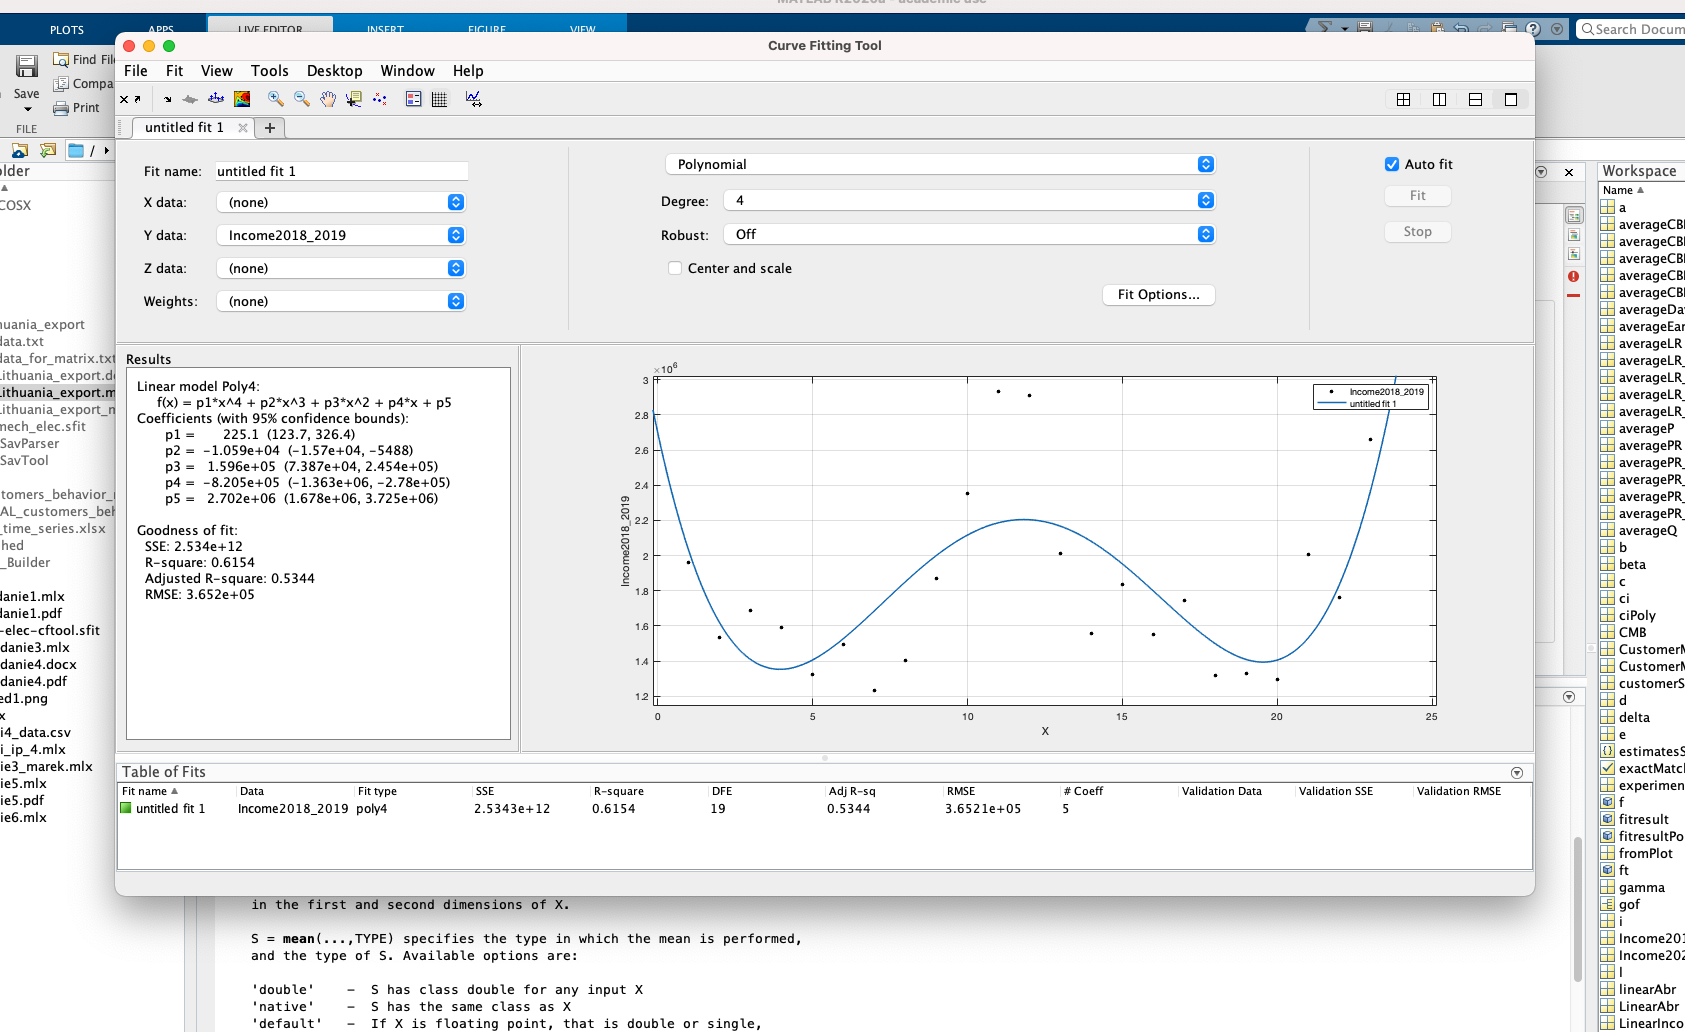
\includegraphics[width=100mm]{cftool.png}
    \end{center}
    \caption{Fitting the data with cftool~\cite{luarn}}
    \label{cftool}
\end{figure}\\
Then to calculate aberration we read the predicted results from the plotted models results as shown on figure~\ref{predict}.
\begin{figure}[h!]
    \begin{center}
        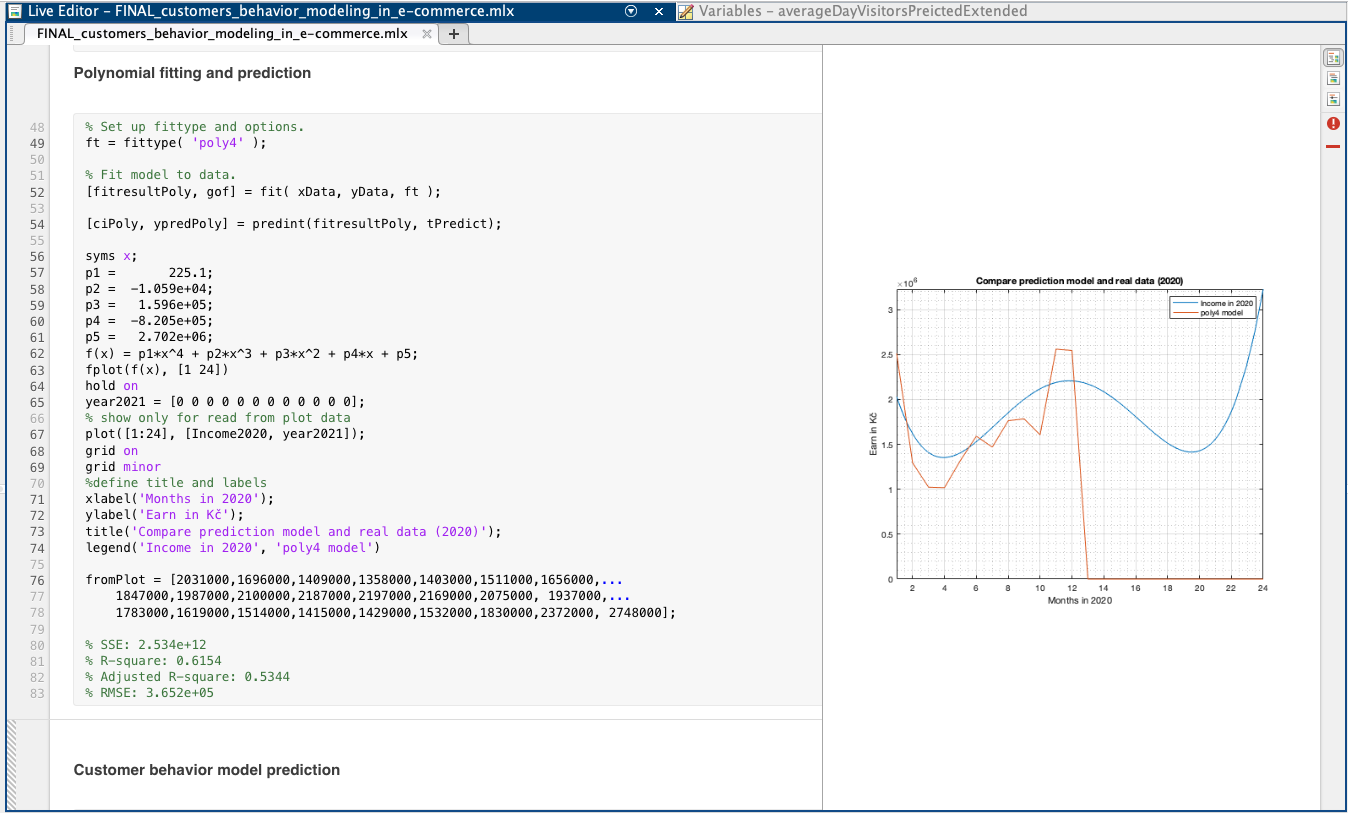
\includegraphics[width=90mm]{predict.png}
    \end{center}
    \caption{Predict income data in live script~\cite{luarn}}
    \label{predict}
\end{figure}\\
\\
Prediction from Customer behavior HMM was made 10 times by default, but this number of cycle run can be easy set in the script.
The final result is arithmetic mean from this prediction which is ten times run to minimize random deviation.
For modeling and dynamic prediction Live scripts Controls are used so in the script we are able to easily set all
constants to model to simulate different situations.
See the dynamic function of our prepared model on figure~\ref{app}.
\begin{figure}[h!]
    \begin{center}
        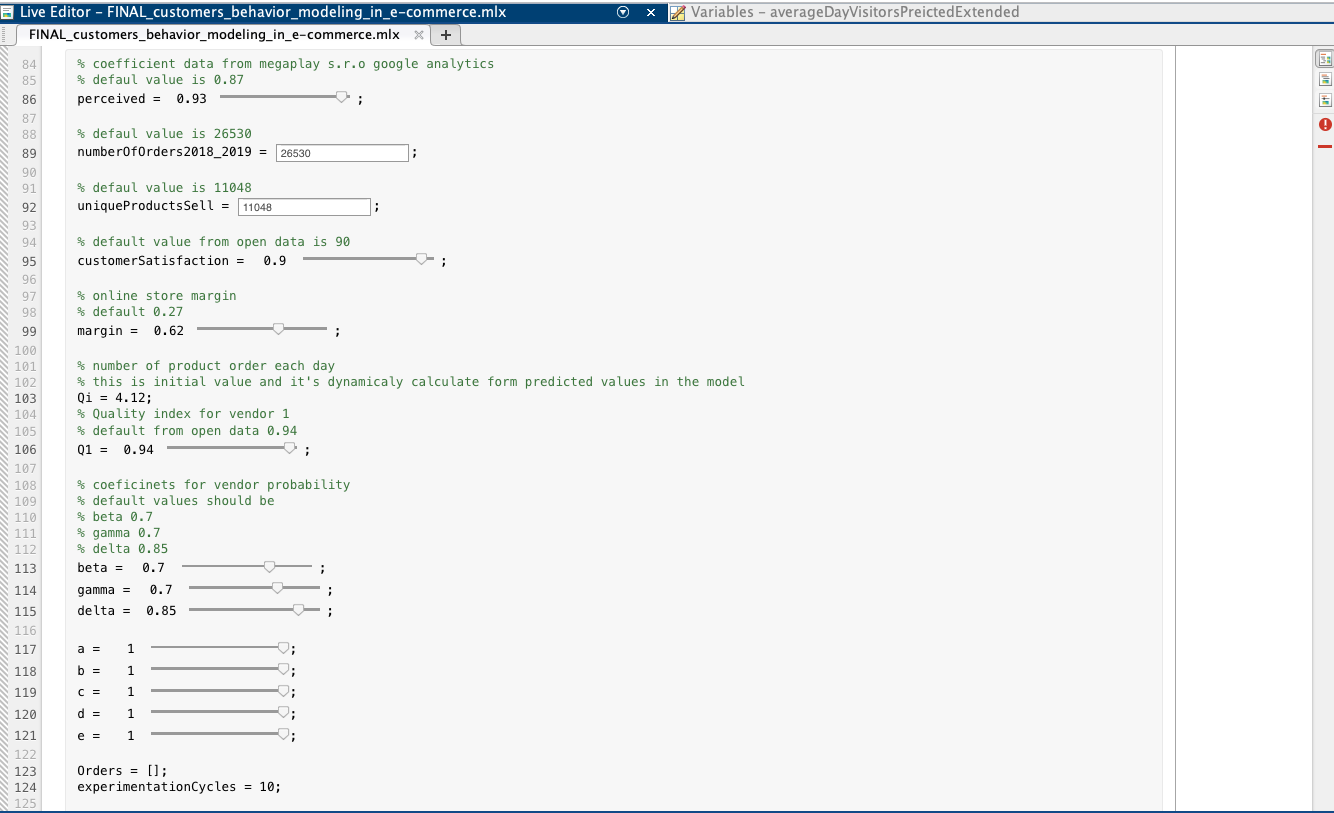
\includegraphics[width=90mm]{app.png}
    \end{center}
    \caption{Live Script application to dynamically set weights and constants for model}
    \label{app}
\end{figure}\\
This precalculated data entered calculation loop.
Next loop reads the value of predefined number of customers in each period and simulates the virtual customer behavior in order process.
This feature gives us ability to easily simulate our model in a different situation.
Lets see some modeled situation in appendix section~\ref{apendixc}.
That results are described in the final summary~\ref{summary} same as results from previous regression models.
